\documentclass[11p]{article}
\usepackage[document]{ragged2e}
\usepackage{amsmath}
\usepackage{amssymb}
\usepackage{tcolorbox}
\usepackage{graphicx}
\usepackage{amsfonts}
\usepackage{caption}
\usepackage{subcaption}
\usepackage{lipsum}
\usepackage[normalem]{ulem}
\usepackage{amsbsy}
\usepackage{wrapfig}
\usepackage{listings}
\usepackage{color}
\usepackage{graphicx}

\usepackage{setspace}

\def\p{\partial}
\def\nl{\newline}
\def\bb{\bigbreak}

\def\ra{\rightarrow}
\def\rai{\rightarrow\infty}
\def\Ra{\Rightarrow}
\def\ra{\rightarrow}


\overfullrule0pt \hoffset=0cm
\parskip=4pt
\parindent=0pt
\baselineskip=20pt

\usepackage[a4paper,margin=.5in,footskip=0.4in]{geometry}


\begin{document}
	
	\title{Limit Order Book Final Report}
	\author{u6680348}
	
    \addtocontents{toc}{\setcounter{tocdepth}{1}}
    
    \maketitle

 
\section{Overview}
A limit order book is a series of data structures and algorithms that allow a stock-market exchange to process and match buy and sell orders. A typical limit order book (LOB) will process upward of 200,000 - 300,000 orders a second, with investors relying on updated price information on a millisecond basis. This makes the speed of this application and subsequently the correct data-structures and algorithms extremely crucial for a successful implementation of an LOB. Orders come in 3 categories:  “buy”, “sell” or “delete”.  When someone makes a buy-order, they are making an offer to buy a stock at a certain price, for example \$13.  If another person makes an order to sell a stock for \$13 or more, then this constitutes a match and the orders are executed.  A delete order simply locates the original order you made and deletes it.  The role of a LOB is to store these orders, make comparisons between them, execute the orders and provide statistics on all trades.   \bigbreak

The three functionalities of this software are all managed through the main/user\_interaction.cpp file. These three functionalities are defined as:
\begin{enumerate}
    \item Order information storage: Used to store order information and provide quick access to the two price-order trees (primary datastructure: hashtable)
    \item Price comparisons and storage: Compares buy/sell orders and executes them if there is a match (primary datastructure: redblack tree)
    \item Statistics and order logging: When an order is made or executed, the data is logged in a logging file. This data is then used to provide traders with price statistics, something that is used frequently in market exchanges/platforms (primary algorithm: random quick sort).
\end{enumerate}
A more in depth overview of these functionalities can be found in the subsequent sections.

\subsection*{Program Overview}
The 3 functionalities join together to form one large functionality, namely processing market orders. The following is a summary of how the algorithm works, followed by a diagram to assist with understanding. \nl
\textbf{Making a buy/sell order}:
\begin{itemize}
    \item[$>>$]Prior to the orders being placed, a buy tree, a sell tree, the hashtable, the order log and statistics class are instantiated.
    \item[$>>$] A new order is read in through a text file and the `newOrder()' function is called. The buy and sell red-black trees are then referenced to determine whether the current buy order is greater than the minimum sell order (or sell order with max buy order).
    \item[$>>$]  If yes then the buy and sell orders are executed and the trade information is sent to the logging file / statistics class. The orders are deleted from the data structures.
    \item[$>>$] If no, the function sends the order to the hash table.
    \item[$>>$] The hash table then inserts the order into the appropriate red-black tree and stores a pointer to this node.
\end{itemize}

\textbf{Order Statistics} \nl
The order statistics provide information on the maximum bid offer, average price for the day, top 75\% of trades and other useful information for traders. To make an `order' for statistics the "getStatistics()" functionality is called with the choice of statistics wanted (or "all" for all data). The function firstly sorts all the orders that have been placed up until that point and then obtains and prints the appropriate statistics.

\bigbreak
\textbf{Order Logging} \nl
Although this is not one of the functionalities, it is useful for checking everything is working. Because the first two functionalities purely maintain orders, they run under-the-hood and do not have any output. The orderlog provides a way to view what orders have been made and what orders are being processed and executed by the hashtable and red-black trees. When any order is made or executed, you can specify whether to print to an orderlog or not. If yes, then the output will be sent to an order-log text file for viewing (see README.md for more information on this). The order log text file format is as follows: date, time, price, buy ID, sell ID.
\bigbreak

\textbf{Assumptions on inputs, memory and operating system} \nl
The size of the input files will range from 10,000 to 500,000. Although the typical amount of orders on a normal day or trading will be around 200,000, we cannot exclude the cases when some popular event triggers larger than normal trading volume (number of orders). Because of these outlier cases, example files with up to 500,000 elements will be used. \bigbreak

The amount of memory required for this application could be as little as 4GB, however because speed is the most important factor here it could be as large as 8-16GB. The largest factor that needs to be considered here is the size of the hash table. In all the experimental analysis, a hash-table of size 16 million (see section 3 for an explanation of this number) and a computer with 16GB of RAM was used. Using the local mac activity monitor, the larger cases used approximately 70\% of this memory. Because of this, I will assume that software is run using 16GB of allocated memory. \bigbreak

This application will run on a mac or linux based operating system. It has not been tested on a windows machine. \bigbreak


\textbf{Limit Order Book Overview} \nl
Please note that because OrderLog is not one of the three functionalities, it has been omitted from the below graph.
\begin{figure}[hbt!]
	\centering
	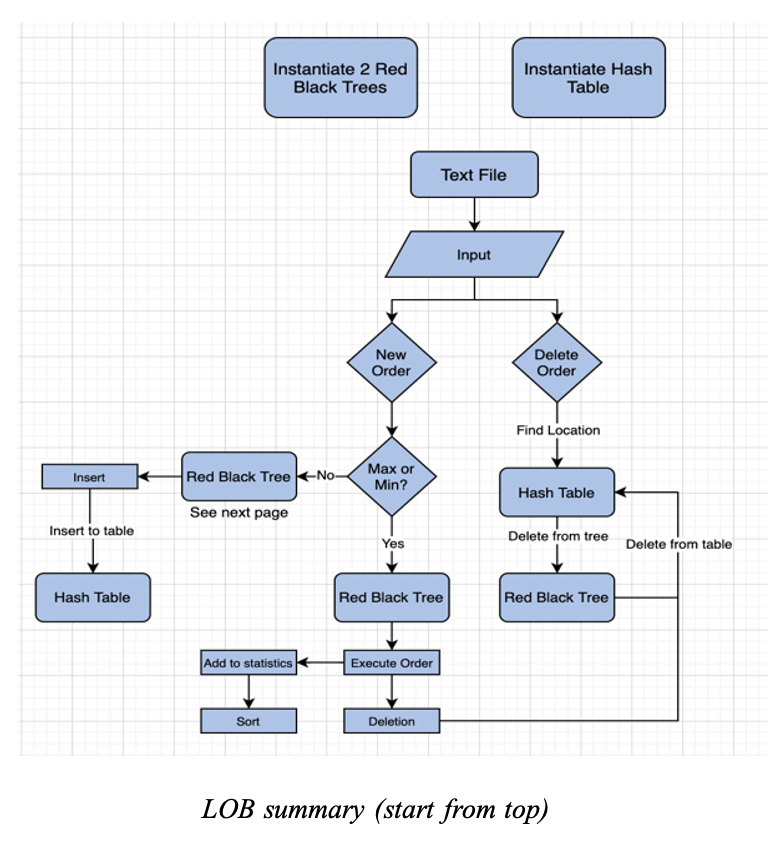
\includegraphics[width=.6\linewidth]{overallprogram.png}
\end{figure}


\pagebreak





\section{Order Statistics - Random Quick Sort}
\subsection{Overview and suitability}
Market exchanges and trading platforms often provide trading statistics to their users. These statistics include things like the maximum bid offer, average price for the day, top 15\% of trades et cetera. In order to obtain this sort of information, the trading data needs to first be sorted. Random quick sort was the sort most applicable for a number of reasons. Firstly, although a non-comparison based sort would have been preferable due to the faster worst-case run-time they were not compatible with this data for the following reasons:
\begin{itemize}
    \item[--] Count Sort: requires a small distribution of numbers 0 to k. The pricing data variance could be upward of \$100.
    \item[--] Bucket Sort: requires a uniform distribution of inputs between 0 and 1. Pricing data varies outside of the 0 to 1 range. This could be remedied by normalising the data then re-normalising it afterwards, however this would counteract the speed benefit of using this sort.
    \item[--] Radix Sort: Requires a constant number of decimal places. User input may vary from for example 10.0 to 10.0001, depending on the popularity of the stock (share) in question. Padding all numbers with say 8 zeros to make them all equal would lead to the sort spending most of it's time sorting zeroes. This was not efficient so the idea was discarded.
\end{itemize}
The reason for choosing random quick sort, over any of the other comparison based sorts was due to the worst-case run time being very unlikely. By randomising the pivot point of quicksort, the chances of the algorithm running in the worst-case $\mathcal{O}(n^2)$ is unlikely to occur. Given it also has a worst-case expected run-time of $\mathcal{O}(nlog(n))$, it is an ideal comparison based sort.
Also, a stable algorithm was also not necessary for this functionality as the statistics provided are not dependent on time of insertion. Therefore random quick sort was the most compatible choice of sorting function for this functionality.

\subsection{Theoretical Time Complexity Analysis}
When getStatistics() is called using the argument `all' to specify you want all statistics, a few methods are called. It firstly sorts all of your data then calls the Statistics class to obtain the volume (number) of orders, max, min and upper, middle and lower quartiles of executed trades. Because the data is sorted, these statistics only require accessing particular indexes in the list and doing an arithmetic operation on the element found. Therefore all of these functions, except for random quick sort run in $\mathcal{O}(1)$ time. Random quick sort is more complicated and is analysed below:



Random quick sort has two major components to analyse, the partition location and the comparisons in the partition functions for-loop. The rest of the algorithm runs in constant time, so these can be considered later. 
\subsubsection{Expected time complexity}
The for loop (line 16) of the partition function is where the majority of operations occur. To determine how many times this runs we will first define the random indicator variable $X_{ij}$ as:
\begin{equation*}
    I\{i,j \}=
    \begin{cases}
    1 & \text{if } e_i \text{ and } e_j \text{ are compared} \\
    0 &  \text{otherwise}
    \end{cases}
    \end{equation*}
Where $e_i$ and $e_j$ are two elements of the list we are sorting. The expected total number of comparisons to completely sort an array is therefore:
\begin{align*}
    &E\big[\sum_{i=1}^{n-1} \sum_{j = i+1}^{n} X_{ij}\big] = \sum_{i=1}^{n-1} \sum_{j = i+1}^{n} E[X_{ij}] \\
    &= \sum_{i=1}^{n-1} \sum_{j = i+1}^{n} Pr(e_i \text{ being compared to } e_j)]
\end{align*}

To determine $Pr(e_i \text{ being compared to } e_j)$ we firstly need to find the probability of any element being chosen as a pivot. This is important because in the random quick sort algorithm, two elements will only ever be compared if one of these is chosen as a pivot. Given there are j - i + 1 elements, and the random function is uniform, the probability of $e_i$ being chosen as a pivot is $\frac{1}{j - i + 1}$ and similarly for $e_j$. Therefore the probability of either being chosen is the sum of these, or $\frac{2}{j-i+1}$. Plugging this into the summation above we get:
$$\sum_{i=1}^{n-1} \sum_{j = i+1}^{n} \frac{2}{j-i+1}$$
Letting the value m be defined as j - i this can be rewritten as:
\begin{align*}
    \sum_{i=1}^{n-1}& \sum_{m=1}^{n-i} \frac{2}{m+1} < \sum_{i=1}^{n-1} \sum_{m=1}^{n} \frac{1}{m} \\
    &=  \sum_{i=1}^{n-1} 2(log_e(n) + \gamma) \ \text{ where } \gamma \text{ is Euler's constant } \\
    & = \sum_{i=1}^{n-1} 2(\frac{logn}{log(e)} + \gamma) < cnlog(n) = \mathcal{O}(nlog(n))
\end{align*}
Therefore the worst-case expected time compelexity of random quick sort is $\mathcal{O}(nlog(n))$. \bigbreak

To find the best-case and subsequently a tight bounded expected time complexity we analyse the scenario when the random pivot is always chosen to be the element in the middle of the array. This will cause the array to be split in half at each iteration. Once split in half, all elements are guaranteed to be compared with the pivot (hence the $\Theta(n)$ below) This can be written as the recurrence:
$$T(n) = 2T\big( \frac{n}{2}\big) + \Theta(n)$$

Using the masters theorem we see that the f(n) above ($\Theta(n))$ is equal to $\Theta(n^{log_2(2)}) = \Theta(n)$. Therefore a = 2 and b = 2. This satisfies case 2 of masters theorem, giving the best case expected time complexity of $\Theta(nlog(n))$. \bigbreak

Given the best case expected time complexity is $\Theta(nlog(n))$, and the worst case expected time complexity is $\mathcal{O}(nlog(n))$, i.e the worst case equals the best case, it must be that the expected time complexity of this functionality is:
$$\Theta(nlog(n))$$

\subsubsection{Worst-case time complexity}
The worst-case time occurs when the random pivot is chosen to be the last element or first element of the array every time. In this case, the size of the partitioned array would only decrease by 1 with every Randompartition recusive call. In the first call n elements would be iterated over. In the second call n-1 would be iterated over. It would take a total of n recursive calls to reach 1 element, giving us the run-time equation:
$$T(n) =  cn + \sum_{i=1}^n c(n-i) = cn + c\big( \frac{n^2 + n}{2}\big)$$
Taking the limit $\lim_{n\to \infty} \frac{T(n)}{n^2}$ we find that the worst-case time complexity is $\mathcal{O}(n^2)$. As mentioned above, the rest of the functionality only takes $\mathcal{O}(1)$ time, thus does not affect the $\mathcal{O}(n^2)$ worst-case.

\pagebreak

\subsection{Empirical Time Complexity Analysis}
Earlier we made the assumption that the total number of elements running through the algorithm at any point in time will be approximately 200,000. As a precautionary measure, inputs from size 10,000 to 500,000 were tested during this experimental analysis. To test the sorting time complexity, various sized vectors of prices were inputed into the sorting function. This was repeated 15 times on each test file, and then the average time was taken. At each iteration, the vector was reshuffled to prevent the algorithm sorting an already sorted array. A table of results and the corresponding time vs input size graph is shown below:

\begin{figure}[hbt!]
	\centering
	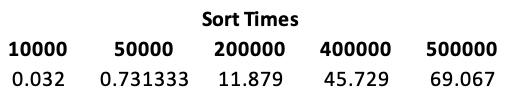
\includegraphics[width=0.4\linewidth]{experimental_results/sorttable.png}
\end{figure}

\begin{figure}[hbt!]
	\centering
	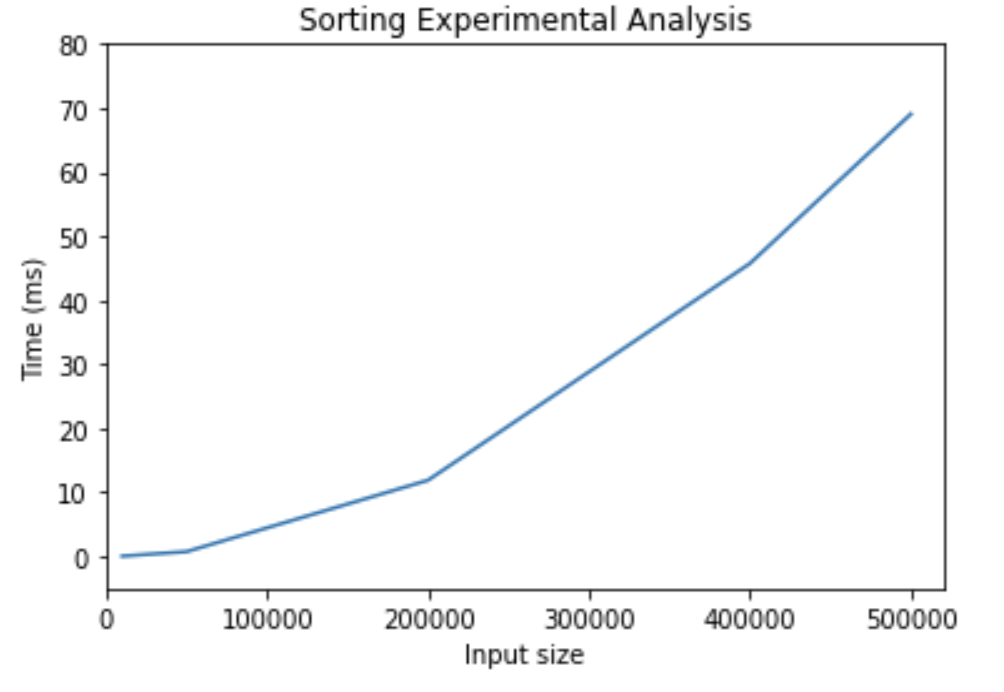
\includegraphics[width=0.4\linewidth]{experimental_results/sortGraph.png}
\end{figure}
\subsubsection{Data analysis and comparison to theoretical time complexity}

Because the data that results from fitting a curve to the theoretical time complexity will have different units to the results of the data found in the experimental analysis, it will be useful to compare the percentage change as inputs is scaled between the two. Using percentage change will allow us to compare the experimental data against the theoretical using the same units.The results of the comparison are shown below (fitted data in orange, actual data in blue):

\begin{figure}[hbt!]
	\centering
	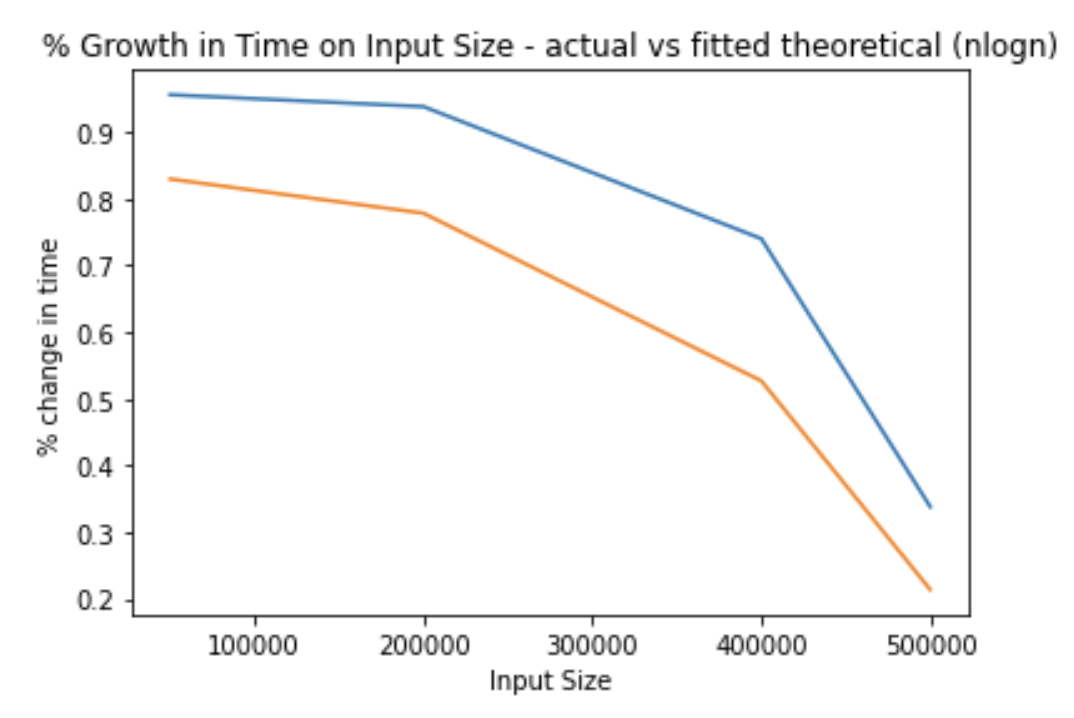
\includegraphics[width=0.4\linewidth]{experimental_results/sortComp.png}
\end{figure}

As you can see, the experimental data closely resembles the theoretical time complexity $\Theta(nlogn)$. The reason the two graphs are downward sloping is due to the distribution of input size; i.e it increases extremely fast from 10,000 to 50,000 to 200,000, then slowly increases from there to 400,000 and 500,000. What is important here is the shape of both graphs. The only large difference is that the actual data looks to be multiplied by some constant scalar, increasing it at all points. This is expected as our theoretical time complexities omit any constant multiplication. Overall we can conclude that the experimental data matches the theoretical analysis conducted earlier.

\pagebreak


\section{Hash-Table}
\subsection{Overview and suitability}

When a buy or sell order is made by a customer, the details of the trade must be stored. Due to speed being the most important factor of this application, constant time insertion/deletion/search is the main priority. Also, because there will be many duplicates among order prices, finding a way to store data by the unique order ID string generated for each order would be extremely useful. These two requirements make a hash-table a very suitable data structure. The only other alternative with constant access time is an array, however due to the IDs being in a random string format, a hash-function/table was required to hash these IDs to indexes. Also, because collisions may occur when hashing, a collision method was needed ... something an array cannot handle.\bigbreak
\textbf{Order IDs} \nl
When an order is made, it is assigned a unique ID string. This string is modified mix of a version 1 and 4 universally unique identifier. The compenents of each version used in this implementation was the date-time from a Version 1 UUID and randomness from Version 4 UUID. These two components were adapted and used to create a unique ID that had a specific date-time for descriptive purposes. \nl

\textbf{Hash Function} \nl
The hash function used for the LOB is a modified version of the FNV-1a hashing algorithm. The reason for using this is primarily it's simplicity and effectiveness in avoiding collisions. The simplicity of the function comes from it's use of primary machine instructions (bit shift, multiply and add); given this implementation is only 6 lines, the speed of the hash function is O(length of the string). When analysing the collision rate of the hash function, it was approximately 10\% when filling the table up to a load factor of 20\%. \nl

\textbf{Load Factor} \nl
As mentioned in the introduction, an LOB will contain at maximum 200,000 to 300,000 elements. The reason it doesn't exceed this, despite there being many orders is that the elements are constantly being deleted (due to buy/sell orders matching and being executed). Because of this, setting the table size to a particular value and leaving it for the duration of the orders is fine. For all experimental tests, the table was set to $2^{24}$. This ensured the load factor was as low as possible throughout the entire order cycle. Although the memory requirements of this large of a table may be high, because speed is a higher priority, this trade-off was made. Because of this, no table-resizing functionality is needed.\nl

\textbf{Collision Resolution Method} \nl
Because resizing it not used, chaining is used as the method for handling collisions. Although this will slightly affect speed, the time-taken to use open addressing and handle resizing the table would be much larger than the difference between handling the occasional collision using open addressing rather than chaining.  \nl

\textbf{Table Contents} \nl
Each entry in the table contains a price, the order ID and a pointer to the corresponding price node in the red-black tree. Because deletion from the RB trees are just as frequent as insertion, it also has to be quick and scaling the tree every time a deletion is required would be time consuming. To solve this, a pointer to the tree nodes is stored in the hash-table; when an order is executed, an $\mathcal{O}(1)$ hash is made to find the entry and the tree node is immediately found and removed, preventing the $\mathcal{O}(log(n))$ worst case tree traversal to find the node. \nl


\subsection{Theoretical Time Complexity Analysis}
\textbf{Assumption - Uniform hash function}:\nl
The modified FNV-1a hash function that was used, together with the modified uuid ID generation create a hash function that is generally uniform. To test this, a hash-table of size 4000 was created and 1000 elements were inserted; of these, 930 were sent to unique locations in the hash table. Increasing the size of the hash-table further decreased collisions, however at the expense of memory. The theoretical analysis will therefore be conducted under the assumptions that both the input and output are uniformly distributed, a fair assumption given these results. \bigbreak 
Also, the functionality as a whole, excluding the hash-table methods run in $\mathcal{O}(1)$ time. Starting from the newOrder() function in user\_interaction.cpp, the functionality begins by calling this function then checking over a number of conditional statements. These conditional statements then make a call to the hash table, thus only requiring a constant time worth of operations prior to the hash table methods. Because constant time does not affect asymptotic time complexity, this component of the functionality will be assumed to be incorporated in the analysis below. The remaining portion of this functionality, i.e. the hash table component is analysed below. 

\pagebreak
\subsubsection{Insertion and Deletion - Worst Case}
Although the worst-case can be easily avoided, it is useful to analyse as a metric for what could go wrong if the hash-table is not set up with the right size. The worst case insertion occurs when all entries into the table are placed in the same slot. This may occur from a very small hash-table or a poorly designed hashing function. In this case, insertion would require firstly passing the ID through the hash function which takes $\mathcal{O}(1)$ and then scaling a linked list through all the elements previously inserted, causing a run-time of $\mathcal{O}(n)$. \nl
Similarly, deleting would also require $\mathcal{O}(n)$ in the worst case, as searching for the element to delete could require scaling an entire linked list to find the element to delete. Add this to the rest of the functionality $\mathcal{O}(n) + \mathcal{O}(1)$ and we get a worst-case run time of $\mathcal{O}(n)$ for the entire functionality.

\subsection{Expected Run Time}
\subsubsection{Insertion - Expected Time}
Firstly, it will be useful to note that the expected time to insert an element will have the same expected time complexity as searching for an element in a hash table without success. Suppose we are inserting a new element into the table: we use the hashing function and find that an element already exists in that bucket so the algorithm traverses the linked-list chain until it finds an empty space. This is akin to a search which will go through the same steps until it finds an empty spot and returns an unsuccessful error message \dots the algorithm in both cases is just searching for an empty bucket or spot in a linked list. \nl

A uniform hashing function implies that the probability of inserting a value into a particular bucket is $\frac{1}{m}$ (where m = table size). To analyse the expected run-time let the random indicator variable $X_a$ be defined as:
\begin{equation*}
I\{a \}=
\begin{cases}
1 & \text{if } h(a) = h(i) \\
0 & \text{if } h(a) \ne h(i)
\end{cases}
\end{equation*}
For element `a' being inserted into the table and element `i' previously inserted. Then the expected value of $X_a$ occurring $E[X_a] = Pr(h(a) = h(i)) \cdot 1 + Pr(h(a) \ne h(i)) \cdot 0 = \frac{1}{m}$. The probability of the new element `a' colliding with any of the n i's inserted previously is therefore:
$$E[\sum_{i=1}^n X_i] = \sum_{i=1}^nE[ X_i] = \sum_{i=1}^n \frac{1}{m} = \frac{n}{m}$$
This is the current load factor of the hash table with size m. The expected time complexity of an unsuccessful search and therefore insertion is thus the load factor $\frac{n}{m}$ plus a constant time worth of operations to calculate the hash function i.e.
$$\Theta(\frac{n}{m} + 1) = \Theta({\frac{n + m}{m}}) \text{ or } \Theta(\alpha + 1)  \text{ where } \alpha \text{ is the load factor}$$
Adding this to the constant time worth of operations calculated prior to the hash-function insert being called and we get an expected time complexity for the entire `insert' portion of this functionality as:
$$\Theta(\alpha + 2)$$



\subsubsection{Deletion - Expected Time Complexity}

Similarly to above, deletion will have the same time complexity as a search through the hash table, however this time with a successful outcome. This is because deletion is purely just a search through the table, then a constant time worth of operations to firstly calculate the hashing function and then remove the pointers and values. \nl
Let the random indicator variable $X_a$ (a is the element to delete) be defined as:
\begin{equation*}
    I\{a \}=
    \begin{cases}
    1 & \text{if } h(a) = h(i) \\
    0 & \text{if } h(a) \ne h(i)
    \end{cases}
\end{equation*}
We already found that the probability of $h(a) = h(i) = \frac{1}{m}$. We then calculate the probability of the new value `a' colliding with any previously inserted elements `i' plus the expected number of elements in the linked list at the particular collision, before the value we are looking to delete. This is equivalent to finding all the elements in the linked list that were inserted after the element we are looking to delete: 
$$E\big[\frac{1}{n} \sum_{i=1}^n (1 + \sum_{j = i+1}^n X_{ij}) \big]$$
Using linearity of expectations and expanding out the brackets and sums:
$$ 1 + \frac{1}{n} \sum_{i=1}^n \sum_{j = i+1}^n E[X_{ij}] = 1 + \frac{n}{m} - \frac{1 + n}{2m} = 1 + \frac{n}{2m} - \frac{1}{2m}$$

$$ = 1 + \alpha \frac{1}{2} - \frac{n}{2mn} = 1 + \alpha \frac{1}{2} - \alpha \frac{1}{2n}$$
Where $\alpha$ is again the load factor. Taking the limit as n goes to infinity of this equation we find the time complexity is $\Theta({\alpha})$. Therefore the total time complexity for the `deletion' portion of this functionality is this plus the constant time operations for computing the hash function, plus the constant time worth of operations made prior to calling the hash delete i.e.
$$\Theta(\alpha) + \Theta(1) + \Theta(1)= \Theta(2 + \alpha)$$

\pagebreak

\subsection{Empirical Time Complexity Analysis}
Similarly to the random quick sort experimental analysis, input sizes ranging from 10,000 to 500,000 were tested. In order to test the hash table independently of the other functionalities, lines 86 and 144 of hashtable.hpp were commented out to prevent the hash table insert/delete calling the red-black tree insert/delete. Given we will always know the maximum size of the input, the hash table can be initially set to have a very low load factor. In this analysis, the size was set to 16 million; given we have access to the memory, this is perfectly reasonable. The table's insert/delete and search times were then tested on random inputs of varying sizes.A results table for the analysis (in milliseconds) is shown below:


\begin{figure}[hbt!]
	\centering
	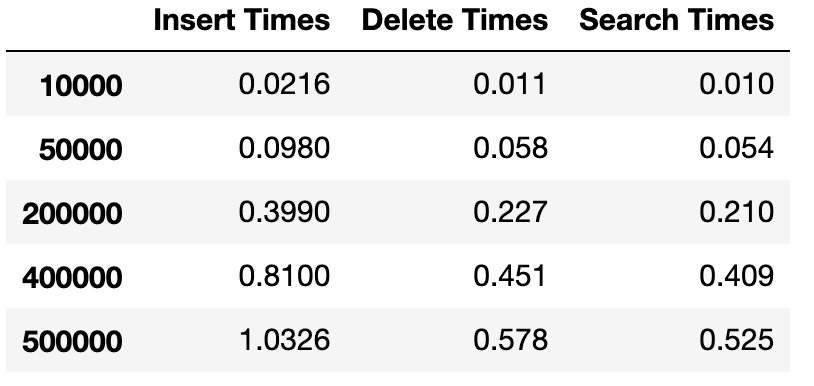
\includegraphics[width=0.3\linewidth]{experimental_results/htabletable.png}
	\caption{Hash table experimental analysis: Input size vs time in ms}
\end{figure}

\begin{figure}[hbt!]
	\centering
	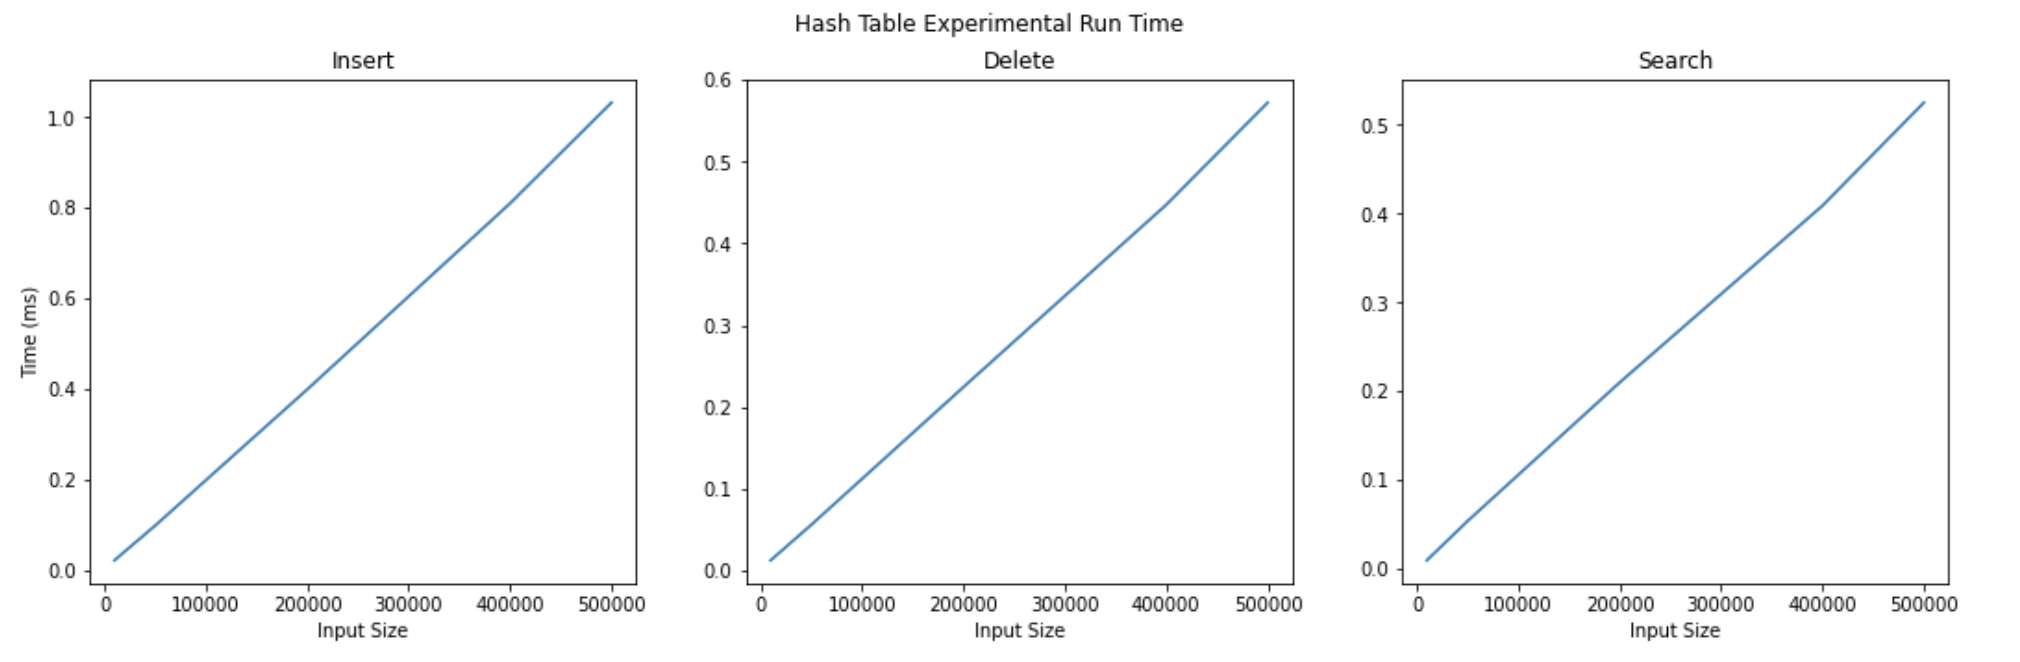
\includegraphics[width=0.9\linewidth]{experimental_results/htablegraph.png}
	\caption{Hash table overall run-time - note the differences on y-axis}
\end{figure}
\subsubsection{Data analysis and comparison to theoretical time complexity}
The graph above is obviously linear, however it is only showing overall run-time. To show time complexity and compare it against the derived theoretical complexity, we need to show how much the time increases per operation, given an increase in input size. Again, similar to the reasoning mentioned in \textit{section 2.3.1}, the percentage growth in time is useful in comparing results measured in different units.  To do this, the percentage increase in time taken to perform each operation were graphed against a constant time worth of time per operation (here the constant time was set to 1). This graph is shown below. When comparing the actual percentage change in time measured (orange line), with the fitted results (blue line), you can see that they are very similar. This implies that as input size increases, the time taken to conduct each operation is constant (as found in the theoretical analysis); the theoretical finding is aligned with the experimental finding. The curve is downward sloping as the size of the percentage increase of inputs is decreasing (i.e. the percentage change between 500,000 and 400,000 inputs is smaller than the percentage change between 50,000 and 10,000). Overall we can conclude that the time complexity of the hash table operations are $\mathcal{O}(1)$.


\begin{figure}[hbt!]
	\centering
	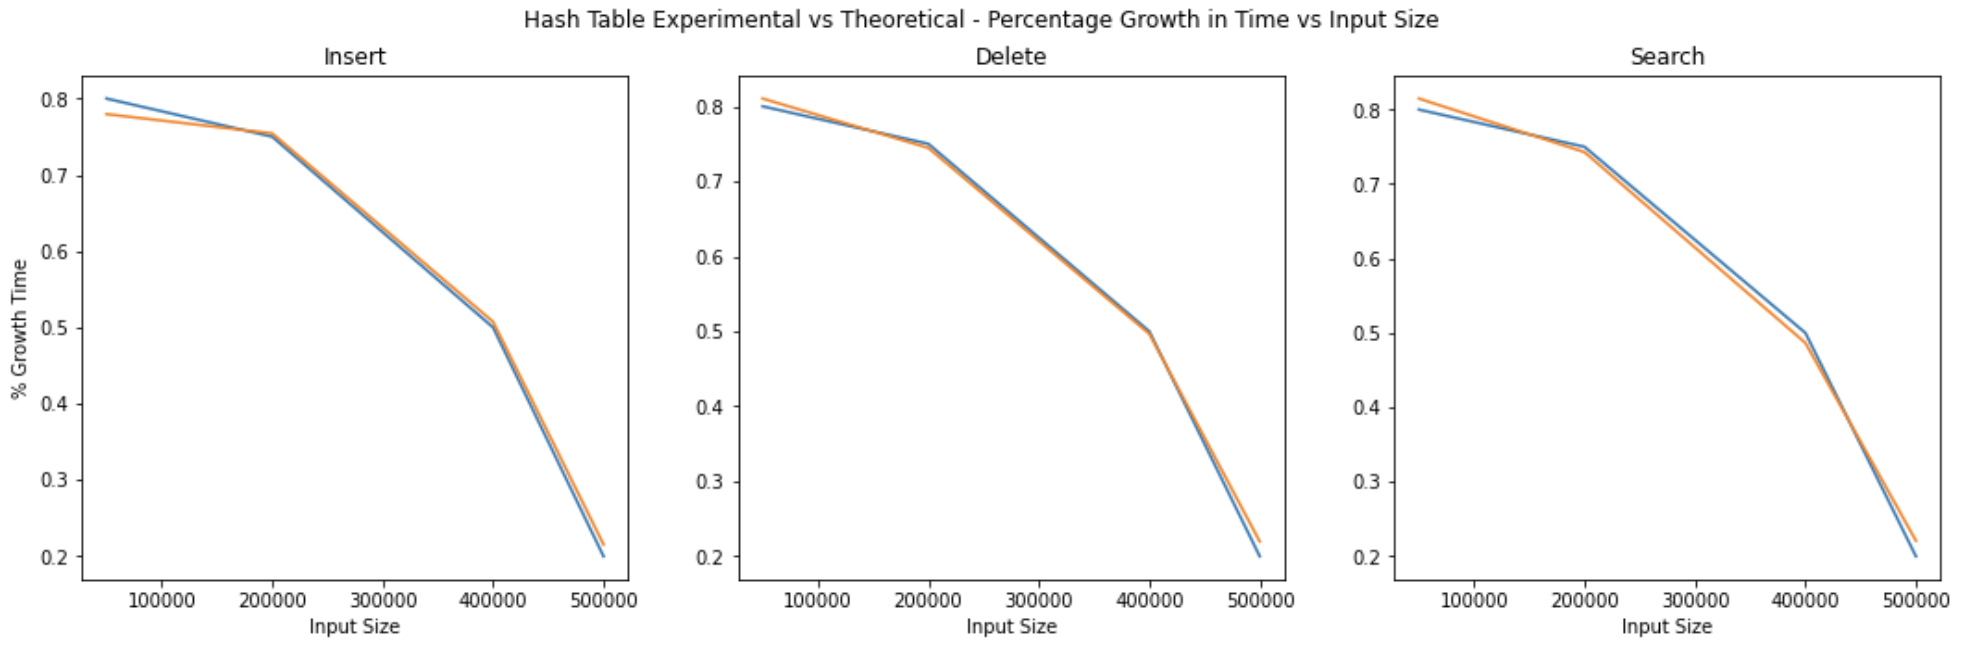
\includegraphics[width=0.9\linewidth]{experimental_results/htablecomp.png}
\end{figure}

\pagebreak

\section{Red-Black Tree}
\subsection{Overview and suitability}
The primary task of a limit-order-book is insertion and deletion of orders. A common LOB may process up to 200,000 orders a second so speed in this area is the priority. A self-balancing tree to store and compare prices is an obvious choice as insertion/deletion worst case is $\mathcal{O}(logn)$ rather than a BST which is $\mathcal(n)$. The reason for choosing a red-black tree is the more relaxed balancing constraints (in comparison to an AVL tree), requiring less rotations during the insertion/deletion process. This may cause slower look-up times, however because the location of each node will be stored in the hash-table, this will not affect the speed of the algorithm at all. The reason for storing prices here as well as in the hash-table is that the hash table does not conduct any `sorting' that a binary tree (RB tree) will. This is important when comparing all buy orders to all the sell orders. Because both the red-black trees and a hash table have components that were necessary for the entire application, both were used, however the primary `price' storage is done by the two trees (one buy and one sell tree). 



\textbf{Optimisations:} \nl
My tree has a few distinct differences compared to a regular RB tree. The first is that  each node stores a queue. If multiple ID's with the same price (value) get inserted, the ID's will just get appended to the back of one of the previous node's queue with the same price. If two orders with the same price are made, the second will not require the tree to undergo a fix-up, allowing the speed of the algorithm to be significantly faster and also require less memory creating new nodes. The second difference is that a pointer to the maximum buy node (in the buy tree) and minimum sell node (in the sell tree) is stored in the tree at all time. Because an order executes when the max buy is greater than the min sell, having quick access to these prices is mandatory and this change allows for this. Because the locations of the nodes are stored in the hash-table, a search function was not required for the tree.

\textbf{Nodes} \nl
Each node contains 7 pieces of information: A pointer to the parent, left child and right child, a boolean representing the colour, a double for order price, a string for the order ID and a queue for order ID. \nl

\subsection{Theoretical Time Complexity Analysis}

When an order is placed, newOrder() firstly accesses a number of elements in the buy and sell tree to determine whether the new trade and an old trade `match' (can be executed). If it does, then an element is deleted from the red-black tree, otherwise the order is inserted into the tree for later comparison. These initial steps, calling newOrder(), accessing the RB tree pointers and conducting a number of conditional checks within the newOrder() and executeorder() functions are all $\mathcal{O}(1)$ time. The only portion of this functionality that does not run in constant time is insertion and deletion from the trees. This is analysed below.



\subsubsection{Insertion - worst-case}
Red-black insertion is comprised of two steps: The binary tree insertion and a fix-up to maintain the RB properties.  Firstly, it will be useful to note that the time-complexity of rotate left and right are O(1). They both perform at most 13 operations, regardless of input size.
\bb
Although the LOB tree has a queue to prevent node restructuring, in the worse case we can assume all prices are distinct and thus the queues are not utilised. \nl

\textit{1. Binary Tree Insertion (lines 35-90):}\nl
Given the red-black tree is a balanced tree it will have height log(n) plus/minus 2, thus traversing the tree using a binary-search will take log(n) multiplied by a constant time. This constant time includes instantiating a node with the specific ID/price, allocating pointers to it's children and parents and colouring the node. Thus the worst-case time complexity for the binary-tree insertion portion is $\mathcal{O}(log(n) \cdot c) = \mathcal{O}(log(n))$. \nl

\textit{2. Fix-up (lines 92-141):} \nl
Firstly, all lines within the while-loop except the 4 cases of rotation run in constant time. We found earlier that the rotations also take $\mathcal{O}(1)$ time.  These rotations will happen at maximum, two times per iteration (if case 2 and subsequently case 3 are triggered), giving the overall run-time of each iteration of the while loop $\mathcal{O}(1)$. \nl
Secondly, lines 105 and 128 (cases 1 and 2) of the while loop set the currnode equal to it's grandparent node. In the worse case, each reassignment is to a red grandparent. In this case the while loop would run until the current node was equal to the node before the root node. Because each iteration assigns the current node to it's grandparent (i.e skips the parent), the number of iterations of the while loop would therefore be half the height of the tree. The height of the tree is $log(n)$, therefore the number of iterations is $\frac{log(n)}{2}$. Therefore, overall fix-up has an overall time complexity of: $$\frac{log(n)}{2} \cdot \mathcal{O}(1) = \mathcal{O}(log(n))$$ \nl
Therefore, for the initial steps of the functionality (calling newOrder, conditionals etc), the BST insert and fix-up, insertion takes at worst:
$$\mathcal{O}(log(n)) + \mathcal{O}(log(n)) + \mathcal{O}(1) = \mathcal{O}(log(n))$$




\subsubsection{Insertion - Best Case}
The best-case would occur when all nodes being inserted are the same price. Because the RB tree node's include a queue for ID's with the same price, the insertion time would be $\Theta(1)$. There would only exist one node (the root node) in the tree and a constant time would be needed to set up the price, ID pair, and another constant time to insert the ID into the root node's queue. Because the queue is simply a linked-list with a pointer to the beginning, the new element can be inserted at the front in $\Theta(1)$ time (just creating a pointer to the next element). Therefore the best case run time is $\Theta(1)$.


\subsubsection{Deletion - Worse Case}
A big difference between the LOB red-black tree and a regular RB tree is that the location of each node is stored in the hash table, thus traversing the tree to find a node isn't needed. We can see that all operations in delete\_price() except delete\_fixup(x) run in constant time. Secondly, all operations in the delete\_fixup while loop are also constant time. Rb\_transplant and both rotations contain only a constant number of operations. \nl

In the worst case, the while loop will iterate a total of log(n) times (height of the tree). This will occur when case 2 of the deletion (lines 247-251) is called every iteration. The while loop will terminate when the current node is red or when the current node equals the root node. Case 2 is the only case where the current node's colour is not changed to red. Therefore, the fix-up and subsequently the deletion portion of this functionality in general has worst case time complexity:
$$\mathcal{O}(log(n)\cdot \mathcal{O}(1) + \mathcal{O}(1)= \mathcal{O}(log(n))$$
Were the $\mathcal{O}(1)$ was added for all the newOrder() operations made before delete is called.
\subsubsection{Deletion - Best Case}
The best-case occurs when the node you are deleting is a red-node at the bottom of the tree. Because the hash-table stores the location to the node on the tree, all that is required for deletion is finding the hash table entry, and then removing the pointers from the previous tree node. No fix-up would be required as the path of black nodes from the root would not change. Therefore, in this case the `delete' portion of this functionality would take a constant time worth of operations $\Theta(1)$ plus the other constant time worth of operations in newOrder() for a total best case deletion of $\Theta(2)$.



\subsubsection{Average-case Run Time - Insertion}
We showed in the previous section that the height of a red black tree in the worse case is log(n). Given it is a balanced tree, it must have a height of log(n) in the best case also. Given this we can say that the expected height of the tree will be $\Theta(log(n))$. Due to the tree allowing for a balance factor of 2, the new node will either be inserted in the second-last layer, the last layer, or on a new layer. Given the second-last layer will be more `full' than the last layer, the probability of the node being inserted in the second-last will be smaller. Given this, let us assume on average it is inserted in the last layer or a new layer with equal probability (Pr = 0.5). Given this, the number of traversals required to reach these layers are $\Theta(log(n))$ and $\Theta(log(n) + 1)$ respectively. \bb

The second thing to analyse is the total number of fix-ups (rotations and colour changes) required after insertion. Because the tree is balanced, and the expected number of black nodes will be half the entire number of nodes (the number of black nodes will most likely be a few more than the red, however given a large tree this difference is negligible ). This property means that similar to the worst-case insertion, the fix-up while loop will have to iterate up the entire tree. Because the while loop skips all the black-nodes, and conducts either 1 or 2 rotation per cycle, we can deduce that the expected number of iterations is $2 \cdot \frac{log(n)}{2}$ or $1 \cdot \frac{log(n)}{2}$. As constants are irrelevant in asymptotic analysis, we can conclude that the expected time complexity for the fixup is $\Theta(log(n))$. \bigbreak

Therefore, the overall expected time complexity is $\Theta(log(n))$ for the tree traversal plus $\Theta(log(n))$ for the fix-up, plus $\mathcal{O}(1)$ for the constant time operations at the beginning of the functionality (the newOrder() call). Together this equals $\Theta(log(n))$. 


\subsubsection{Average-case Run Time - Deletion}
As mentioned in `Deletion - Worst Case', the location of the node is known by the hash table prior to deletion, therefore there is no traversal necessary. The expected time complexity of delete fix-up will be derived similarly to the expected insertion complexity. Because both insertion and deletion consist of a while loop that will only break when the root is reached or the grandparent node's colour is different from it's own, they will both have the same time complexity. The only difference is that deletion has a larger number of constant time operations, however this is not relevant in asymptotic time complexity. Including the newOrder() constant time operations, deletion has an expected time complexity of $\Theta(log(n))$.




\subsection{Empirical Time Complexity Analysis}
As mentioned in \textit{section 2.2.2} deletion of the red-black tree does not require firstly traversing the tree; this was resolved by storing the location in the hash table to be accessed in $\mathcal{O}(1)$ time. Testing red-black node deletion thus involves firstly retrieving the node location from the hash table using the hash-search and then removing it from the tree and performing the fix-up. \textit{Section 4.4} timed the hash function insert and delete with the red-black tree line of code commented out. Because the rb-tree insert and delete cannot be tested independently of the hash-table, timing the entire insert and delete of the hashtable/rbtree (without commenting out the lines of code mentioned in section 4.4) will be conducted. The results of the hashtable insert/delete (section 4.4) will then be taken away from these results , giving us the time of just the red-black tree component. A table of these results (in milliseconds) is shown below.


\begin{figure}[hbt!]
	\centering
	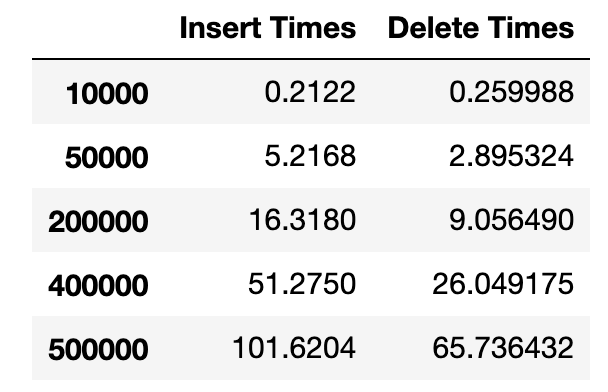
\includegraphics[width=0.3\linewidth]{experimental_results/rbtreetable.png}
	\caption{Red black tree experimental analysis: Input size vs time in ms}
\end{figure}
\begin{figure}[hbt!]
	\centering
	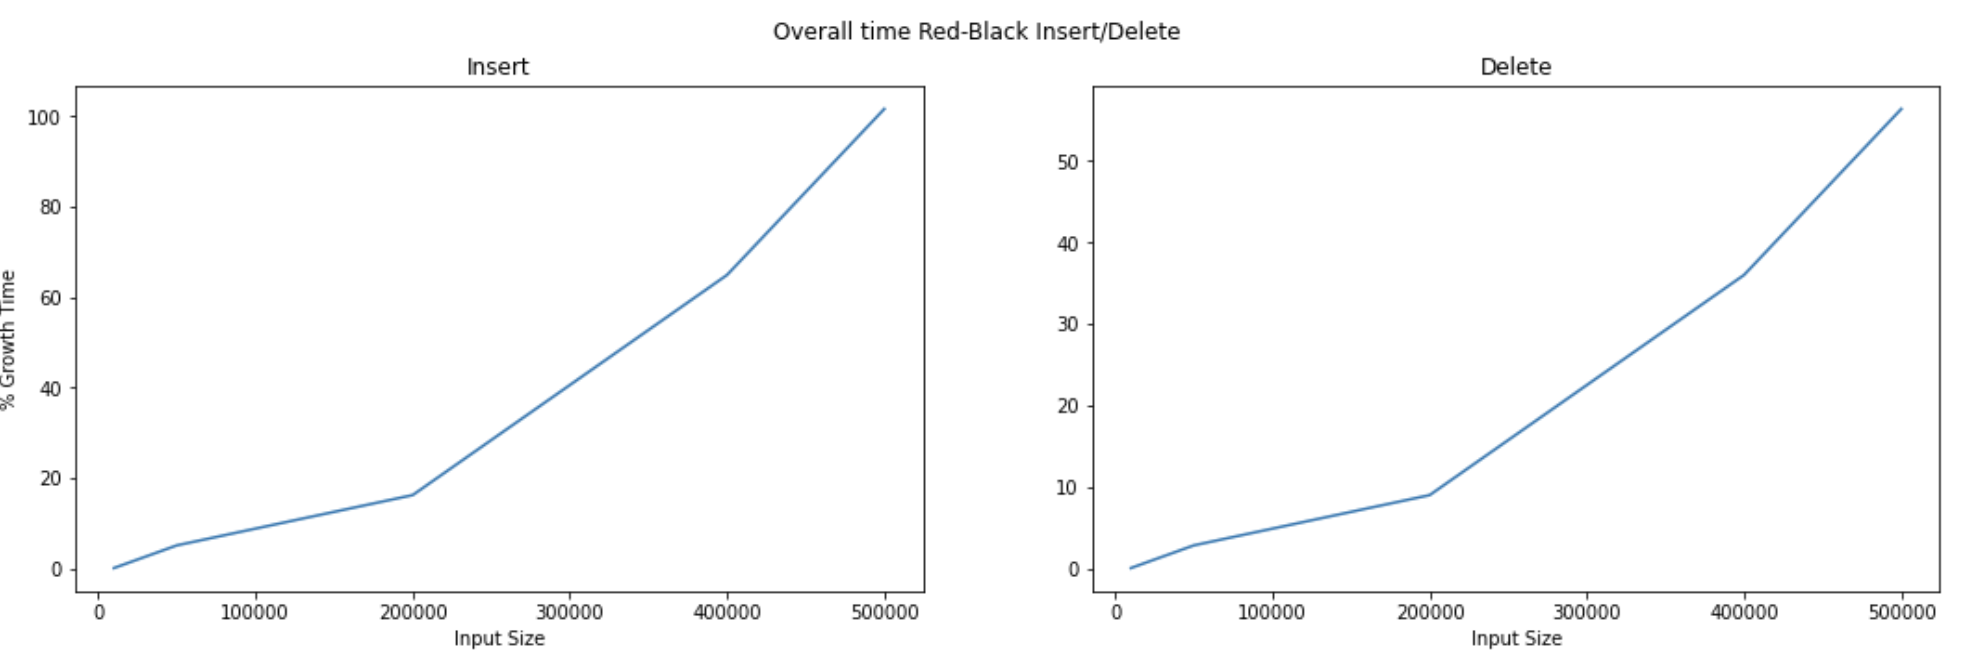
\includegraphics[width=0.6\linewidth]{experimental_results/rbgraph.png}
\end{figure}

\subsubsection{Data analysis and comparison to theoretical time complexity}
Similar to the empirical analysis for \textit{section 2.3.1}  and \textit{section 3.4.2}, percentage growth in time over inputs was used to compare the empirical results to the theoretical time complexity. The results of this are shown below. The reason for the downward sloping curves is also explained in these previous sections. \nl
Comparing the two curves, we can see that the orange (actual data) is steeper than the theoretical results, implying that the time taken to insert and delete elements grows faster with input size; this flattens off as inputs get very large. Therefore, although insert and delete may not have a time complexity of $O(log(n))$, the actual complexity will be very close to this. Also, the actual data seems to be scaled by some constant scalar factor (this explains the height difference between the two curves), this was to be expected as big-O time complexity omits any constants.
\begin{figure}[hbt!]
	\centering
	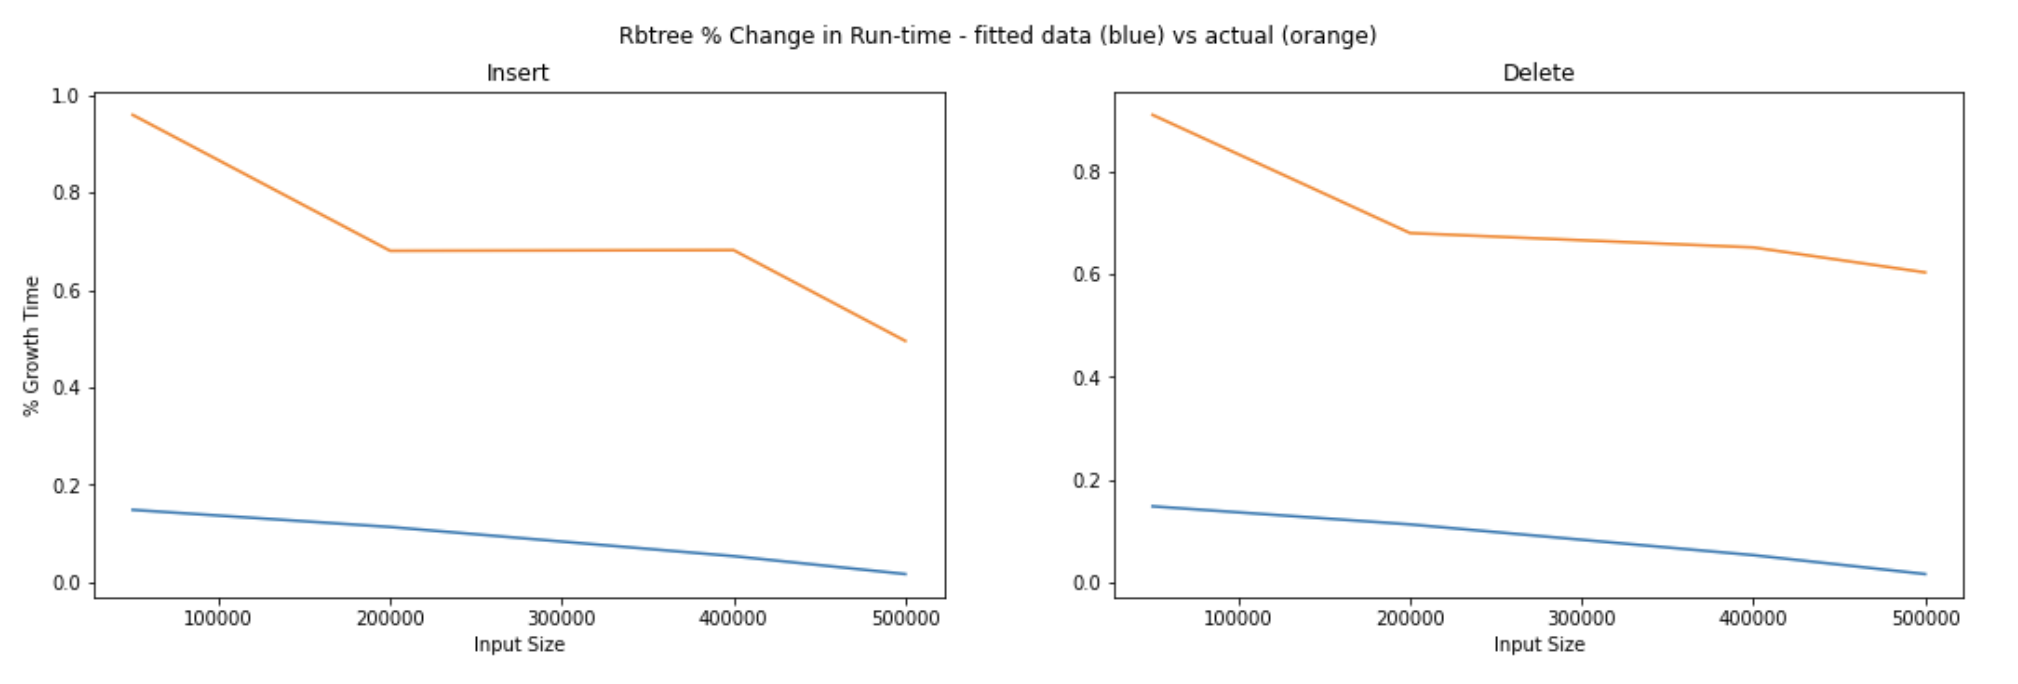
\includegraphics[width=0.7\linewidth]{experimental_results/rbtreecomp.png}
	\caption{Red black tree experimental analysis: \% Change in run-time vs Input size}
\end{figure}

\pagebreak




\end{document}